\documentclass[dvipsnames, svgnames, x11names]{beamer}

\usetheme{mytheme}
\usetikzlibrary{tikzmark}
\special{dvipdfmx:config z 0} %取消PDF压缩，加快速度，最终版本生成的时候最好把这句话注释掉

%封面
\title{单室模型}
\author{张斌}
\institute[理工系]{河北农业大学 理工系}
\date{\the\year 年 \the\month 月}



\begin{document}

	
	\begin{frame}
		\titlepage
		\thispagestyle{empty}
		\addtocounter{framenumber}{-1}
	\end{frame}





\begin{frame}{}
	\begin{center}
		{\Huge \cbf{目 \ 录}}
	\end{center}
	\tableofcontents[subsectionstyle=hide/hide/show]
	\thispagestyle{empty}
	\addtocounter{framenumber}{-1}
\end{frame}

\begin{frame}
    \frametitle{单室模型}
    单室模型是一种最简单的房室模型，它把整个机体视为一个房室，药物进入体内后迅速分布于体液和全身各组织，并在体内各组织之间迅速达到动态平衡，药物在各组织之间的转运速率处于“均一状态”。
    
    \begin{itemize}
      \item 体内过程符合单室模型的药物称为单室模型药物 。
      \item 单室模型并不意味机体中各组织或体液内的药物浓度完全相等 ， 但是药物在机体各组织中的转运速率相同或者相近 ， 机体各组织中的药物浓度能随血浆药物浓度的变化而平行发生变化 。
      \item 药物从体内按一级过程消除
    \end{itemize}
    
\end{frame}


\section{静脉注射给药动力学}

\subsection{血药浓度的经时变化}

\begin{frame}
    \frametitle{模型的建立}
    单室模型药物静脉注射给药后 ，药物迅速完成分布 ，只有消除过程 ，如图所示 。 药物在体内的消除为一级速率过程 。
\begin{center}
    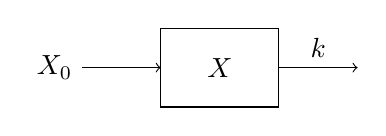
\begin{tikzpicture}
        \draw[->] (0,0) node[left]{$X_0$} --  (1,0);
        \draw (1,-0.5) rectangle (2.5,0.5) node[midway] {$X$};
        \draw[->] (2.5,0) -- (3.5,0) node[above,midway]{$k$};
    \end{tikzpicture}
\end{center}
$X_0$为给药剂量；$X$为体内药量；$k$为一级消除速率常数

单室模型药物静注给药后 ， 药物的消除速率与体内该时刻药物的量成正比 ：
\[
    \frac{\mathrm{d}X}{\mathrm{d}t}=-kX
\]
上式中 ， $\frac{\mathrm{d}X}{\mathrm{d}t}$表示体内药物的消除速率；负号表示体内药量随时间延长不断减少 。
\end{frame}


\begin{frame}
    \frametitle{血药浓度与时间的关系}
    微分方程式$\frac{\mathrm{d}X}{\mathrm{d}t}=-kX$经拉氏变换 ， 得 ：
    \[
        s\overline{X}-X_{0}=-k\overline{X}
    \]
    \[
        \overline{X}=\frac{X_{0}}{s+k}
    \]
    上式中 ， $s$为拉氏运算子；$\overline{X}$为原函数$X$的拉氏变换 ， 即$X$的象函数

    再经拉氏逆变换后得到体内药量变化的函数表达式：
    \[
        X = X_0e^{-kt}
    \]
    根据定义$X=VC$，可将体内药量变化的函数表达式改述为血药浓度与时间的关系式：
    \[
        C = C_0e^{-kt}
    \]
\end{frame}


\begin{frame}
    \frametitle{总消除速率常数$k$与初始血药浓度$C_0$的计算}
    \begin{minipage}{0.7\linewidth}
        将$C = C_0e^{-kt}$两边取对数，得
        \[
            \ln C=-kt+\ln C_{0}
        \]
        取常用对数，得
        \[
            \lg C=-\frac k{2.303}t+\lg C_0
        \]
        上述方程表明$\lg C$与$t$呈线性关系，该直线的斜率为$-k/2.303$，截距为$\lg C_0$。
        
        当单室模型药物静脉注射给药以后 ， 测得不同时间 $t_i$的血药浓度$C_i(\mathrm{~i=1~,2~,\cdots,n~})$， 以$\lg C$ 对$t$作图 ，从其斜率我们可求得消除速率常数$k$，从其截距我们可求得给药后瞬时间的血药浓度$C_0$。
    \end{minipage}\hfill
    \begin{minipage}{0.25\linewidth}
        \begin{figure}[htpb]
            \centering
            
\includegraphics[width=\linewidth]{浓度时间曲线}
            
\includegraphics[width=\linewidth]{对数时间图}
        \end{figure}
    \end{minipage}
\end{frame}


\begin{frame}
    \frametitle{半衰期$t_{1/2}$的计算}
    将$t=t_{1/2},C=C_{0}/2$代入$\ln C=-kt+\ln C_{0}$，得
    \[
        \ln\frac{C_{0}}{2}=-kt_{1/2}+\ln C_{0}
    \]
    \[
        t_{_{1/2}}=\frac{\ln2}k\approx\frac{0.693}k
    \]
    可见，如果药物在体内呈一级消除过程，其半衰期与给药剂量和给药途径无关 。

    由于半衰期比消除速率常数更为直观，故临床上多用$t_{1/2}$来反映药物消除的快慢，它是临床制定给药方案的主要依据之一。

    \begin{question}
        药物从体内消除90\%所需的时间？
    \end{question}
    \vspace{-7pt}
\end{frame}

\begin{frame}[t]
    \frametitle{消除若干百分数所需的时间}    
    药物从体内消除若干百分数所需的时间 （ 亦可描述为所需半衰期的个数 ） 可用下法计算 ：
    \[
        t=\frac{\ln C_{0}-\ln C}{k}=\frac{\ln(C_{0}/C)}{\ln2/t_{1/2}}=\frac{\ln(C_{0}/C)}{\ln2}t_{1/2}
    \]
    消除90\%，$(C=C_{0}/10)$，所需时间为 3.32$t_{1/2}$
    \begin{table}
        \centering
        \begin{tabular}{ccc|ccc}
            \bottomrule
            半衰期个数 & 剩余(\%) & 消除(\%) & 半衰期个数 & 剩余(\%) & 消除(\%) \\ \hline
            0 & 100 & 0 & 4 & 6.25 & 93.75 \\ 
            1 & 50 & 50 & 5 & 3.12 & 96.88 \\
            2 & 25 & 75 & 6 & 1.56 & 98.44 \\
            3 & 12.5 & 87.5 & 7 & 0.78 & 99.22 \\ \toprule
        \end{tabular}
        \caption{经历若干个半衰期后药物从体内消除的百分数}
    \end{table}
\end{frame}


\begin{frame}[t]
    \frametitle{}
    \begin{example}
        某患者快速静注一单室模型药物 100 mg ， 立即测得血药浓度为 10 mg/ml ， 4 小时后 ，血药浓度为 7.5 mg/ml ，求该药在此患者体内的半衰期 。
    \end{example}
    \pause
    \[
        kt=\ln\frac{C_{0}}{C}
    \]
    \[
        k=0.072(\mathrm{h}^{-1})
    \]
    \[
        t_{1/2}=\frac{0.693}k=\frac{0.693}{0.072}=9.6\mathrm{~(h)}
    \]
\end{frame}


\begin{frame}[t]
    \frametitle{表观分布容积($V$)的计算}
    \[
        V = \frac{X_0}{C_0}
    \]
    
\end{frame}


\begin{frame}[t]
    \frametitle{血药浓度---时间曲线下面积($AUC$)的计算}
    AUC是评价药物吸收程度的一个重要指标，常被用于评价药物的吸收程度。
    \[
        \begin{aligned}
            AUC_{0\to\infty}&=\int_{0}^{\infty}C\mathrm{d}t \\
            &=\int_0^\infty C_0\cdot\mathrm{e}^{-kt}\mathrm{d}t \\
            &=C_0\int_0^\infty\mathrm{e}^{-kt}\mathrm{d}t \\
            &=C_0 \frac{1-\mathrm{e}^{-\infty}}{k}\\
            &=\frac{C_0}k \\
            &=\frac{X_0}{kV}
        \end{aligned}
    \]
    AUC与给药剂量成正比。
\end{frame}


\begin{frame}
    \frametitle{体内总清除率的计算}
    体内总清除率 (Cl) 是指在单位时间内机体能将相当于多少体积血液中的药物完全清除 。
    \[
        \begin{aligned}
            Cl&=\frac{-\mathrm{d}X/\mathrm{d}t}{C} \\
            &=\frac{kX}{C} \\
            &=kV
        \end{aligned}
    \]
    根据$AUC_{0\to\infty}=\frac{X_0}{kV}$，得总清除率的另一个计算公式 ：
    \[
        Cl=\frac{X_{0}}{AUC_{0\to\infty}}
    \]
\end{frame}


\begin{frame}
    \frametitle{总结：动力学参数计算}
    $k$和$C_0$：
    
    以$\ln C$对$t$作图得到一条直线，该直线的斜率为$-k$，截距为$\ln C_0$
    \begin{flalign*}
        & t_{{1/2}}=\frac{\ln2}k & \\
        & V = \frac{X_0}{C_0} & \\
        & AUC_{0\to\infty}=\frac{C_0}k=\frac{X_0}{kV} & \\
        & Cl=kV=\frac{X_{0}}{AUC_{0\to\infty}} & 
    \end{flalign*}
\end{frame}


\begin{frame}[t]
    \frametitle{}
    \begin{example}
        给某患者静脉注射某单室模型药物 ， 剂量 1050 mg ， 测得不同时刻血药浓度数据如下 ：
        \begin{table}
            \centering
            \begin{tabular}{cccccccc}
               \toprule
                $t$(h) & 1.0 & 2.0 & 3.0 & 4.0 & 6.0 & 8.0 & 10.0 \\ \hline
                $C$( $\mu$g/ml ) & 109.78 & 80.35 & 58.81 & 43.04 & 23.05 & 12.35 & 6.61 \\ \bottomrule
            \end{tabular}
        \end{table}
        试求该药物的$k,t_{1/2},V,Cl,{AUC}_{0\to\infty}$以及 12 小时的血药浓度 。
    \end{example}
\end{frame}


\begin{frame}[t]
    \frametitle{}
    \begin{question}
        给某患者静脉注射某单室模型药物 ， 剂量 1500 mg ， 测得不同时刻血药浓度数据如下 ：
        \begin{table}
            \centering
            \begin{tabular}{ccccccccc}
               \toprule
                $t$(h) & 1.0 & 2.0 & 3.0 & 4.0 & 5.0 & 6.0 & 7.0 & 8.0 \\ \hline
                $C$( $\mu$g/ml ) & 154.97 & 120.08 & 93.04 & 72.09 & 55.86 & 43.28 & 33.54 & 25.98 \\ \bottomrule
            \end{tabular}
        \end{table}
        试求该药物的$k,t_{1/2},V,Cl,{AUC}_{0\to\infty}$以及 12 小时的血药浓度 。
    \end{question}
\end{frame}


\subsection{尿药排泄的经时变化}

\begin{frame}
    \frametitle{尿药排泄}
    血药浓度是药物动力学研究以及求算药动学参数的主要方法 。 但在某些情况下血药浓度测定存在困难 ， 例如 ：
    \begin{enumerate}
      \item 血药浓度低 ， 难以准确测定 ；
      \item 血浆成分对药物测定干扰严重 ；
      \item 多次采集血样对人体有损伤 ，患者依从性差 。 
    \end{enumerate}
    尿液取样方便 ， 对人体无损伤 ， 因而在有些情况下 ， 可采用尿药排泄数据求算药动学参数 。 但是该方法须符合以下条件 ：
    \begin{enumerate}
    \item 大部分药物以原形从尿中排泄 ；
    \item 药物经肾排泄符合一级速率过程 ， 即尿中原形药物产生的速率与体内的药量成正比 。
    \end{enumerate}
    尿药排泄数据处理方法包括速率法 （rate method） 和亏量法 （sigma-minus method） 。
\end{frame}



\begin{frame}
    \frametitle{尿药排泄速率与时间的关系 （ 速率法 ）}
    \begin{minipage}{0.48\linewidth}
        \begin{center}
            \begin{tikzpicture}
                \draw (0,-0.5) rectangle (1.5,0.5) node[midway] {$X$};
                \draw[->] (1.5,0) -- (3,0) node[above,midway]{$k_\mathrm{e}$} node[right]{$X_\mathrm{u}$};
                \draw[->] (0.75,-0.5) -- (0.75,-1.5) node[right,midway]{$k_{\mathrm{nr}}$} node[below]{$X_{\mathrm{nr}}$};
            \end{tikzpicture}
        \end{center}
    \end{minipage}\hfill
    \begin{minipage}{0.48\linewidth}
        $X$为体内药量 ；

        $k_\mathrm{e}$为肾排泄速率常数 ；
        
        $k_{\mathrm{nr}}$为非肾途径消除速率常数 ；
        
        $X_\mathrm{u}$为尿中原形药物累积量 ；
        
        $X_{\mathrm{nr}}$为非肾途径排泄的原形药物累积量
    \end{minipage}

    \smallskip
    药物在体内的排泄如图所示 。 大部分药物在体内主要通过肾脏排泄 ， 尿中原形药物的产生不是恒速的 。 尿中原形药物产生的速率与体内的药量$X$和药物的肾排泄速率常数$k_\mathrm{e}$密切相关。

    肾排泄速率常数反映了药物经肾消除的快慢 ， 而药物总的消除速率常数$k$应是$k_\mathrm{e}$与$k_{\mathrm{nr}}$之和 ， 即 $k= k_\mathrm{e} + k_{\mathrm{nr}}$。
\end{frame}


\begin{frame}
    \frametitle{尿药排泄速率与时间的关系 （ 速率法 ）}
    静脉注射单室模型药物 ， 原形药物经肾排泄的速率可用微分方程表示为 ：
    \[
        \frac{\mathrm{d}X_{\mathrm{u}}}{\mathrm{d}t}=k_{\mathrm{e}}X
    \]
    dX
    式中 ， $\frac{\mathrm{d}X_{\mathrm{u}}}{\mathrm{d}t}$为原形药物经肾排泄速率 ；$X_{\mathrm{u}}$为$t$时刻尿中原形药物累积量 ； $X$为$t$时刻体内药物量；$k_{\mathrm{e}}$为肾排泄速率常数 。

    将$X = X_0e^{-kt}$代入，得
    \[
        \frac{\mathrm{d}X_{\mathrm{u}}}{\mathrm{d}t}=k_{\mathrm{e}}X_0e^{-kt}
    \]
    \begin{minipage}{0.48\linewidth}
        两边取常用对数 ， 得 ：
    \[
        \lg\frac{\mathrm{d}X_{\mathrm{u}}}{\mathrm{d}t}=-\frac{k}{2.303}t+\lg(k_\mathrm{e}X_0)
    \]
    \end{minipage}\hfill
    \begin{minipage}{0.48\linewidth}
        两边取自然对数 ， 得 ：
    \[
        \ln\frac{\mathrm{d}X_{\mathrm{u}}}{\mathrm{d}t}=-kt+\ln(k_\mathrm{e}X_0)
    \]
    \end{minipage}
    
\end{frame}


\begin{frame}
    \frametitle{尿药排泄速率与时间的关系 （ 速率法 ）}
    \begin{minipage}{0.48\linewidth}
        \begin{figure}[htpb]
            \centering
            
\includegraphics[width=\linewidth]{尿药排泄}
        \end{figure}
    \end{minipage}\hfill
    \begin{minipage}{0.48\linewidth}
        以$\lg\frac{\mathrm{d}X_{\mathrm{u}}}{\mathrm{d}t}$对$t$作图， 可以得到一条直线。 通过直线的斜率即可求出药物的总消除速率常数$k$。

        直线在纵轴的截距等于$\lg(k_\mathrm{e}X_0)$。 若设该截距为 $\lg{I_0}$ ， 则可求出肾排泄速率常数$k_\mathrm{e}$：
        \[
            k_\mathrm{e} = \frac{I_0}{X_0}
        \]
    \end{minipage}
\end{frame}


\begin{frame}
    \frametitle{尿药排泄速率与时间的关系 （ 速率法 ）}
    $\frac{\mathrm{d}X_{\mathrm{u}}}{\mathrm{d}t}$为$t$时刻的瞬时尿药排泄速率 ， 而尿药浓度只能反映集尿期间的累积排泄量 ， 因此$\frac{\mathrm{d}X_{\mathrm{u}}}{\mathrm{d}t}$无法准确获得 。 实际工作中采用集尿时间间隔$(\mathrm{~}t_\mathrm{i}\rightarrow t_{\mathrm{i+1}})$内的平均尿药排泄速率$\frac{\Delta X_\mathrm{u}}{\Delta t}$代替$\frac{\mathrm{d}X_{\mathrm{u}}}{\mathrm{d}t}$， 以集尿期的中点时间$t_\mathrm{c}$。代替$t$， 即将集尿时间段内的平均尿药排泄速率 ， 近似地看作该段集尿时间内中点时间的瞬时尿药排泄速
    率 。 于是：
    \[
        \begin{aligned}
            \lg\frac{\Delta X_{\mathrm{u}}}{\Delta t}&=-\frac{k}{2.303}t_{\mathrm{c}}+\lg(k_{\mathrm{e}}X_{0}) \\
            \ln\frac{\Delta X_{\mathrm{u}}}{\Delta t}&=-kt_{\mathrm{c}}+\ln(k_{\mathrm{e}}X_{0})
        \end{aligned}
    \]
    式中 ， $\Delta t$为集尿时间 ； $\Delta X_{\mathrm{u}}$为该集尿时间段内排泄的原形药物量 ； $t_{\mathrm{c}}$为集尿期的中点时间 。
\end{frame}


\begin{frame}
    \frametitle{尿药排泄速率与时间的关系（速率法）}
    以$\lg\frac{\Delta X_{\mathrm{u}}}{\Delta t}$对$t_{\mathrm{c}}$作图时 ， 实验数据常因测定误差出现较大的散乱波动 ， 偏离直线较明显 ， 也就是说 ， 速率法对实验测定误差敏感 。 另外 ， 采用尿排泄速率获取药物动力学参数时 ， 收集尿样的时间间隔对药物动力学参数的准确性影响较大。
    \begin{table}
        \centering
        \begin{tabular}{cccc}
            \bottomrule
            时间间隔 & ~~$t_{1/2}$~~ & ~~2$t_{1/2}$~~ & ~~3$t_{1/2}$~~ \\ \hline
            误差 & 2\% & 8\% & 19\% \\ \toprule
        \end{tabular}
    \end{table} 
    因此 ， 应合理设计收集尿样的时间间隔 ， 收集尿样时间间隔一般控制在 2 个半衰期以内较为合适 。 若药物半衰期很短以致于无法在小于 2 个半衰期的时间间隔内收集尿样时 ， 则最好采用相等的集尿时间间隔 。
\end{frame}


\begin{frame}[t]
    \frametitle{}
    \begin{example}
        某单室模型药物给患者静脉注射 200 mg 后 ， 定时收集尿液 ， 测得尿药累积排泄量$X_{\mathrm{u}}$如下表 ， 试求该药的$k$，$t_{1/2}$和$k_\mathrm{e}$值 。（速率法）
        \small{
        \begin{table}
            \centering
            \begin{tabular}{ccccccccccccccccccc}
                \bottomrule
                $t$(h)& 0 & 1 &  2 & 3 & 6 &  12 & 24 & 36 & 48  & 60 & 72  \\ \hline
                $X_{\mathrm{u}}$(mg)& 0 & 4.02 & 7.77  & 11.26 & 20.41 &  33.88 & 48.63 & 55.05 & 57.84  & 59.06 & 59.58 \\ \toprule
            \end{tabular}
        \end{table}}
    \end{example}
\end{frame}


\begin{frame}
    \frametitle{尿药排泄量与时间的关系（亏量法）}
    尿药排泄速率法中 ， 数据波动性大 ， 有时难以准确估算药物的消除速率常数 。 为克服这一缺点 ， 可采用亏量法 。

    对$\frac{\mathrm{d}X_{\mathrm{u}}}{\mathrm{d}t}=k_{\mathrm{e}}X$作拉普拉斯变换，
    \[
        S\overline{X}_{\mathrm{u}}=k_{\mathrm{e}}\overline{X}
    \]
    将$\overline{X}=\frac{X_0}{S+k}$代入，整理得
    \[
        \overline{X}_{\mathrm{u}}=\frac{k_{\mathrm{e}}X_0}{S\left(S+k\right)}
    \]
    应用拉氏变换表解出${X}_{u}$ ：
    \[
        X_{\mathrm{u}}=\frac{k_{\mathrm{e}}X_{0}}{k}(1-\mathrm{e}^{-kt})
    \]
\end{frame}


\begin{frame}
    \frametitle{尿药排泄量与时间的关系（亏量法）}
    \begin{minipage}{0.43\linewidth}
        \begin{figure}[htpb]
            \centering
            
\includegraphics[width=\linewidth]{尿排泄量}
        \end{figure}
    \end{minipage}\hfill
    \begin{minipage}{0.55\linewidth}
        当$t \rightarrow \infty $时 ，$e^{-kt}{\rightarrow}0$， 故最终经肾排泄的原形药物总量$X_{\mathrm{u}}^{\infty}$为 ：
        \[
            X_{\mathrm{u}}^{\infty}=\frac{k_{\mathrm{e}}X_{0}}{k}(1-\mathrm{e}^{-kt_{\infty}})=\frac{k_{\mathrm{e}}X_{0}}{k}
        \]
        
    \end{minipage}
\end{frame}


\begin{frame}
    \frametitle{尿药排泄量与时间的关系（亏量法）}
    用式$X_{\mathrm{u}}^{\infty}=\frac{k_{\mathrm{e}}X_{0}}{k}$减去式$X_{\mathrm{u}}=\frac{k_{\mathrm{e}}X_{0}}{k}(1-\mathrm{e}^{-kt})$：
    \[
        \begin{aligned}
            X_{\mathrm{u}}^{\infty}-X_{\mathrm{u}}&=\frac{k_{\mathrm{e}}X_{0}}{k}-\frac{k_{\mathrm{e}}X_{0}}{k}(1-\mathrm{e}^{-kt}) \\
            &=\frac{k_\mathrm{e}X_0}{k}\mathrm{e}^{-kt}
        \end{aligned}
    \]
    \begin{minipage}{0.48\linewidth}
        两边取常用对数 ， 得 ：
    \[
        \begin{aligned}
            \lg(X_{\mathrm{u}}^{\infty}-X_{\mathrm{u}})&=-\frac{k}{2.303}t+\lg\frac{k_{\mathrm{e}}X_{0}}{k} \\
            &=-\frac{k}{2.303}t + \lg X_{\mathrm{u}}^{\infty}
        \end{aligned}
    \]
    \end{minipage}\hfill
    \begin{minipage}{0.48\linewidth}
        两边取自然对数 ， 得 ：
    \[
        \ln(X_{\mathrm{u}}^{\infty}-X_{\mathrm{u}})=-kt + \ln X_{\mathrm{u}}^{\infty}
    \]
    \bigskip
    \end{minipage}
    
    上两式中$(X_{\mathrm{u}}^{\infty}-X_{u})$称为体内经肾待排泄原形药物量 ， 或称亏量 。
\end{frame}


\begin{frame}
    \frametitle{尿药排泄量与时间的关系（亏量法）}
    \begin{minipage}{0.48\linewidth}
        单室模型药物静脉注射给药后 ， 以体内经肾待排泄原形药物量 （ 亏量 ） 的常用对数$\lg(X_{\mathrm{u}}^{\infty}-X_{\mathrm{u}})$对时间$t$作图 ， 可得到一条直线 ， 该直线的斜率为$-\frac{k}{2.303}$， 截距为$\lg\frac{k_{\mathrm{e}}X_{0}}{k}$。

        \begin{itemize}
          \item 根据斜率 ， 可求出总消除速率常数$k$；
          \item 根据截距 、 静脉注射给药剂量$X_{0}$及$k$可求出肾排泄速率常数$k_{\mathrm{e}}$。
        \end{itemize}
    \end{minipage}\hfill
    \begin{minipage}{0.48\linewidth}
        \begin{figure}[htpb]
            \centering
            
\includegraphics[width=\linewidth]{亏量时间图}
        \end{figure}
    \end{minipage}
\end{frame}


\begin{frame}
    \frametitle{亏量法的特点}
    \begin{enumerate}
      \item 亏量法对药物消除速率的波动和实验测定误差不敏感 ，以$\lg(X_{\mathrm{u}}^{\infty}-X_{\mathrm{u}})$对时间$t$作图时 ， 实验数据点偏离直线不远 ， 比较规则 ， 求得总消除速率常数值较尿药排泄速率法准确 ；
      \item 亏量法中为了得到$X_{\mathrm{u}}^{\infty}$ ， 要求收集尿样的时间要足够长（至少为药物的 7 个半衰期 ） ， 而且不得丢失任何一份尿样数据 。对于半衰期长的药物采用亏量法 ， 完成实验所需要的时间较长 。 相比之下 ， 速率法的集尿时间只需 3 、 4 个半衰期 ， 并且作图确定一个点只需要收集一次尿样 ， 而不必要收集全过程的尿样 。
    \end{enumerate}
\end{frame}


\begin{frame}
    \frametitle{肾排泄率}
    将$X_{\mathrm{u}}^{\infty}=\frac{k_{\mathrm{e}}X_{0}}{k}$整理得
    \[
        \frac{X_\mathrm{u}^{\infty}}{X_{0}}=\frac{k_{\mathrm{e}}}{k}
    \]
    $\frac{k_{\mathrm{e}}}{k}$称为药物的肾排泄率 ， 它反映了药物的肾排泄在药物的总消除中所占的比率 ， 用符号$f_\mathrm{r}$表示：
    \[
        f_\mathrm{r}=\frac{X_\mathrm{u}^{\infty}}{X_{0}}
    \]
    当$k_{\mathrm{e}}=k$时 ， 药物完全以原形经肾排泄 ，$X_{\mathrm{u}}^{\infty}=X_{0}$
\end{frame}


\begin{frame}
    \frametitle{总结}
    单室模型药物静脉注射给药后 ， 可采用三种方法求算药物动力学参数 ： 
    \begin{enumerate}
      \item 以血药浓度的对数对时间作图或进行线性回归 ；
      \item 以平均尿药排泄速率的对数对集尿中点时间作图或进行线性回归 ； 
      \item 以尿药排泄亏量的对数对时间作图或进行线性回归 。
    \end{enumerate}
      这三种方法均可获得直线图或直线回归方程 ，进而根据斜率求出总消除速率常数$k$。研究工作中 ， 可根据实际情况选择 。
\end{frame}


\begin{frame}[t]
    \frametitle{}
    \begin{example}
        某单室模型药物给患者静脉注射 200 mg 后 ， 定时收集尿液 ， 测得尿药累积排泄量$X_{\mathrm{u}}$如下表 ， 试求该药的$k$，$t_{1/2}$和$k_\mathrm{e}$值 。（亏量法）
        \small{
        \begin{table}
            \centering
            \begin{tabular}{ccccccccccccccccccc}
                \bottomrule
                $t$(h)& 0 & 1 &  2 & 3 & 6 &  12 & 24 & 36 & 48  & 60 & 72  \\ \hline
                $X_{\mathrm{u}}$(mg)& 0 & 4.02 & 7.77  & 11.26 & 20.41 &  33.88 & 48.63 & 55.05 & 57.84  & 59.06 & 59.58 \\ \toprule
            \end{tabular}
        \end{table}}
    \end{example}
\end{frame}


\begin{frame}[t]
    \frametitle{}
\begin{question}
    某单室模型药物给患者静脉注射 200 mg 后 ， 定时收集尿液 ， 测得尿药累积排泄量$X_{\mathrm{u}}$如下表 ， 试求该药的$k$，$t_{1/2}$和$k_\mathrm{e}$值 。（速率法和亏量法）
        \begin{table}
            \centering
            \begin{tabular}{cccccccc}
                \bottomrule
                $t$(h)& 0 & 1 &  2 & 3 & 6 &  12\\ 
                $X_{\mathrm{u}}$(mg)& 0 & 4.76 & 9.33 & 13.72 & 25.41 & 43.80 \\ \hline
                $t$(h)& 24 & 36 & 48  & 60 & 72 & 96 \\ 
                $X_{\mathrm{u}}$(mg) & 66.56 & 80.64 & 89.36 & 94.75 & 98.08 & 100.64 \\ \toprule
            \end{tabular}
        \end{table}
\end{question}
\end{frame}


    

\begin{frame}
    \frametitle{肾清除率$(Cl_{\mathrm{r}})$}
    肾清除率 (renal clearance) 系指单位时间内肾将相当于多少体积血浆中的药物全部清
    除 。 肾清除率的单位为 ml/min 或 ml/h 。 药物的肾清除率不超过肾血流量 。

    肾清除率可表示为尿药排泄速率与血药浓度的比值 ， 即 ：
    \[
        \begin{aligned}
            Cl_{_r}&=\frac{\mathrm{d}X_{_u}/\mathrm{d}t}C \\
            &=\frac{k_{\mathrm{e}}X}{C} \\
            &=k_{\mathrm{\mathrm{e}}}V
        \end{aligned}
    \]
    即肾清除率为肾排泄速率常数与表观分布容积的乘积 。 体内所有器官的清除率都可以用相应的消除速率常数与分布容积的乘积来表示 。 药物在体内的总清除率是药物在体内各个器官清除率的总和 。
\end{frame}


\begin{frame}
    \frametitle{肾清除率$(Cl_{\mathrm{r}})$}
    \begin{minipage}{0.6\linewidth}
        $Cl_{_r}=\frac{\mathrm{d}X_{_u}/\mathrm{d}t}C$可整理成：
    \[
        \frac{\mathrm{d}X_\mathrm{u}}{\mathrm{d}t}=Cl_\mathrm{r}C
    \]
    从上式可知 ， 用尿药排泄速率对血药浓度 $C$ 作图 ， 可以得到一条直线 。 在实际工作中 ， 可用实验测得的平均尿药排泄速率$\frac{\Delta X_{u}}{\Delta t}$代替$\frac{\mathrm{d}X_\mathrm{u}}{\mathrm{d}t}$， 对集尿期中点时间$t_{\mathrm{c}}$的血药浓度$C$作图 。 直线的斜率即肾清除率。
    \begin{example}
        某药 $0\sim 0.5$ h内从尿中排出量为37.5 mg, 在0.25 h 时血药浓度为 10 $\mu$g/ml ， 求该药的肾清除率。
    \end{example}
    \end{minipage}\hfill
    \begin{minipage}{0.38\linewidth}
        \begin{figure}[htpb]
            \centering
            
\includegraphics[width=\linewidth]{尿集中期}
        \end{figure}
    \end{minipage}
\end{frame}


\begin{frame}[t]
    \frametitle{}
    \begin{example}
        某药物静脉注射 200 mg 后 ， 定时收集尿液 ， 测得平均尿药排泄速率与中点时间的关系式为
        \[
            \lg\frac{\Delta X_{u}}{\Delta t}=-0.0299t_{\mathrm{c}}+0.6212
        \]
         已知该药属单室模型 ， 分布容积为 30L ， 求该药的 $t_{1/2}$，$k_\mathrm{e}$ ，$Cl_{\mathrm{r}}$及 80h 的累积尿药量 。
    \end{example}
\end{frame}


\begin{frame}[t]
    \frametitle{}
    \begin{example}
        己知磺胺嘧啶半衰期$t_{1/2}=16$ h， 分布容积 V$=20$L ， 尿中回收原形药物 60\%。 求该药总清除率$Cl$， 肾清除率$Cl_{\mathrm{r}}$， 非肾清除率 $Cl_{\mathrm{nr}}$。
    \end{example}
\end{frame}


\section{静脉滴注给药动力学}


\begin{frame}
    \frametitle{静脉输液}
    静脉输液是利用大气压和液体静压原理将大量无菌液体、电解质、药物由静脉输入体内的方法。
    \begin{table}
        \centering
        \begin{tabularx}{\textwidth}{ X | X }
            \bottomrule
            \makecell[c]{优点} &  
            \makecell[c]{缺点} \\ \hline
            易将药物达致疗效浓度，并可持续维持疗效所需的恒定浓度。 & 处理不当易产生全身性或局部性的感染。\\
            对肌肉、皮下组织有刺激的药物可经静脉给予。 & 药物过量或滴注过快，易产生不良反应，甚至危及生命。 \\
            可迅速地补充身体所丧失的液体或血液。 &  持续性的过量输注，易造成循环负荷过重，或电解质失衡。\\
            静脉营养品的输注。 & 医源性疾病的增多。\\ \toprule
        \end{tabularx}
    \end{table}
\end{frame}

\begin{frame}
    \frametitle{能吃药不打针，能打针不输液\link{https://www.nmpa.gov.cn/xxgk/zhcjd/tjzhc/tjzhcyp/20220411091947120.html}}
    \begin{figure}[htpb]
        \centering
        
\includegraphics[width=.45\linewidth]{输液}
    \end{figure}
    \begin{enumerate}
      \item 口服给药途径最常用 ， 相对安全 、 方便 、经济 。
      \item 注射给药途径吸收快 、 药量准确可控 ，但未经过人体天然屏障直接进入体内 ，可引起组织损伤 、 疼痛 、 感染 ， 甚至严重不良反应 。
      \item 盲目输液、过度输液会给患者带来感染、热源、血管内膜损伤等等。
      \item 儿童脏器发育尚未完全 ， 更应谨慎选择给药途径 。
    \end{enumerate}
\end{frame}


\begin{frame}
    \frametitle{模型的建立}
    静脉滴注是以恒定速率向静脉血管内持续给药 。 单室模型药物静脉滴注进入体内 ， 在滴注时间$T$以内 ， 体内同时存在药量增加和药物消除的过程 。 当药物滴注结束后 ， 体内只存在药物的消除过程 。 因此 ， 这种模型包括两个方面 ： 一是药物以恒定速率$k_0$进入体内 ， 二是体内药物以一级消除速率常数$k$从体内消除 。 静脉滴注给药体内过程的模型如下图所示 。
    \begin{center}
        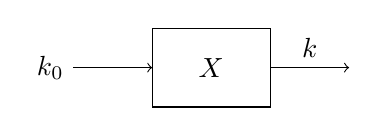
\begin{tikzpicture}
            \draw[->] (0,0) node[left]{$k_0$} --  (1,0);
            \draw (1,-0.5) rectangle (2.5,0.5) node[midway] {$X$};
            \draw[->] (2.5,0) -- (3.5,0) node[above,midway]{$k$};
        \end{tikzpicture}
    \end{center}
    $k_0$为静脉滴注速率；$X$为体内药量；$k$为一级消除速率常数
    \[
        \frac{\mathrm{d}X}{\mathrm{d}t}=k_{0}-kX
    \]
\end{frame}


\begin{frame}
    \frametitle{血药浓度与时间的关系}
    $\frac{\mathrm{d}X}{\mathrm{d}t}=k_{0}-kX$经拉氏变换 ， 得 ：
    \[
        S\overline{X}=\frac{k_{0}}{S}-k\overline{X}
    \]
    整理后 ， 得 ：
    \[
        \overline{X}=\frac{k_{0}}{S(S+k)}
    \]
    用拉氏变换求原函数 ， 得 ：
    \[
        X=\frac{k_{0}}{k}(1-\mathrm{e}^{-kt})
    \]
    将 $X=VC$代入 ， 得到体内血药浓度$C$与时间$T$之间的函数关系式 ：
    \[
        C=\frac{k_{0}}{kV}(1-\mathrm{e}^{-kt})
    \]
\end{frame}


\begin{frame}
    \frametitle{稳态血药浓度($C_\mathrm{ss}$)}
    

    \begin{minipage}{0.53\linewidth}
        在静脉滴注给药初期 ， 血药浓度迅速上升 ， 随着静脉滴注时间的延长 ， 血药浓度上升速度趋于缓慢 ， 当$t\to\infty$时，$e^{-kt}\to0$，$(1 - e^{-kt})\to1$，血药浓度趋于一个恒定浓度 ， 此时的血药浓度值称为稳态血药浓度或坪浓度 ， 用$C_\mathrm{ss}$表示 。
        \[
        C_\mathrm{ss}=\frac{k_{0}}{kV}
        \]
        \begin{itemize}
            \item 稳态血药浓度$C_\mathrm{ss}$与静滴速率$k_{0}$成正比； 
            \item 在达到稳态血药浓度的状态下，药物的静滴速率$k_{0}$等于体内药物的消除速率 。
          \end{itemize}
    \end{minipage}\hfill
    \begin{minipage}{0.43\linewidth}
        \begin{figure}[htpb]
            \centering
            
\includegraphics[width=\linewidth]{稳态浓度}
        \end{figure}
    \end{minipage}
\end{frame}


\begin{frame}
    \frametitle{达稳态所需时间（达坪分数$f_{\mathrm{ss}}$与半衰期$t_{1/2}$的关系 ）}
    血药浓度$C$可用坪浓度$C_\mathrm{ss}$的某一分数来表示 ， 即达坪分数$f_{\mathrm{ss}}$。
    \[
        f_{ss}=\frac{C}{C_{ss}}=\frac{\frac{k_{0}}{kV}(1-e^{-kt})}{\frac{k_{0}}{kV}}=1-\mathrm{e}^{-kt}
    \]
    从上式可见 ， 在相同的滴注时间内 ， 消除速率常数$k$越大 ， 达坪分数$f_{\mathrm{ss}}$越快趋近于 1 ， 达到坪浓度越快 。 也就是说 ， 药物的$t_{1/2}$越短 ， 达到坪浓度越快。

    由上式可求得达到坪浓度某一分数所需要的时间 ：
    \[
        t=-\frac{\ln{(1-f_{_{\mathrm{ss}}})}}k
    \]
    当达到坪浓度某一分数所需要的时间以$n$个半衰期$t_{1/2}$来表示时，可写为 ：
    \[
        n=-\frac{\ln(1-f_{\mathrm{ss}})}{\mathrm{ln2}}=-\frac{2.303\mathrm{lg}(1-f_{ss})}{0.693}=-3.323\lg (1-f_{ss})
    \]
\end{frame}


\begin{frame}
    \frametitle{达坪浓度某一分数所需的半衰期个数}
    不论药物的半衰期$t_{1/2}$长短如何 ， 达到坪浓度某一分数所需要的半衰期$t_{1/2}$的个数都是一样的 。
    \begin{figure}[htpb]
        \centering
        
\includegraphics[width=\linewidth]{半衰期个数}
    \end{figure}
\end{frame}


\begin{frame}[t]
    \frametitle{}
    \begin{example}
        某一单室模型药物，半衰期为 0.5h ， 静脉滴注达稳态血药浓度的 95\%， 需要多少时间 ？
    \end{example}
    
\end{frame}


\begin{frame}[t]
    \frametitle{}
    \begin{example}
        某患者体重50kg，以每分钟20 mg的速率静脉滴注单室模型药物普鲁卡因，问稳态血药浓度是多少？滴注经历10h时的血药浓度是多少？（已知$t_{1/2}=3.5 \mathrm{h}$，$V=$\SI{2}{L/kg}）。
    \end{example}
\end{frame}


\begin{frame}[t]
    \frametitle{}
    \begin{example}
        对某患者静脉滴注单室模型药物利多卡因，已知$t_{1/2}=1.9 \mathrm{h}$，$V=$\SI{100}{L}，若要使稳态血药浓度达到3$\mu$g/mL，静脉滴注速度$k_0$值应为多少？
    \end{example}
\end{frame}


\begin{frame}[t]
    \frametitle{}
    \begin{example}
        利多卡因的有效血药浓度是2.4$\sim$6$\mu$g/mL，如分别以150mg/h和300mg/h的速度进行静脉滴注，问哪种滴注速度合适？如果使患者的稳态血药浓度达到6$\mu$g/mL，则最佳滴注速度是多少？已知$k=1.04 \mathrm{h}^{-1}$，$V=40$L。
    \end{example}
\end{frame}


\begin{frame}
    \frametitle{其他药物动力学参数}
    当静脉滴注一段时间后停止滴注 ， 体内只存在药物的消除过程 。 体内血药浓度的变化情况相当于静脉注射后血药浓度的变化 ， 静脉滴注停止后血药浓度与时间的关系为 ：
    \[
        C=C_0\mathrm{e}^{-kt'}
    \]
    式中 ， $t'$为停止静脉滴注给药后的时间 ；$C$为停止静脉滴注给药后$t'$时刻的血药浓度 ；$C_0$为静脉滴注停止时的血药浓度 。
\end{frame}


\begin{frame}
    \frametitle{稳态后停滴}
    达稳态时 ，$C_0=C_\mathrm{ss}=\frac{k_{0}}{kV}$， 将此式代入式$C=C_0\mathrm{e}^{-kt'}$， 得 ：
    \[
        C=\frac{k_{0}}{kV}\mathrm{e}^{-kt'}
    \]
    取自然对数，得：
    \[
        \ln C=-kt'+\ln\frac{k_{0}}{kV}
    \]
    取常用对数，得：
    \[
        \lg C=-\frac{k}{2.303}t'+\lg\frac{k_{0}}{kV}
    \]
    根据上式 ， 可计算出总消除速率常数$k$及表观分布容积$V$。即在停药后不同时间取血 ，测定血药浓度， 以$\lg C$ 对$t'$作图或进行线性回归，得到一直线或直线回归方程。
\end{frame}


\begin{frame}
    \frametitle{稳态前停滴}
    假设静脉滴注$T$时间后停药， 则静脉滴注$T$时间的血药浓度$C_0$为

    \begin{minipage}{0.48\linewidth}
        \[
            C_0=\frac{k_{0}}{kV}(1-\mathrm{e}^{-kT})
        \]
        代入式$C=C_0\mathrm{e}^{-kt'}$， 得 ：
        \[
            C=\frac{k_{0}}{kV}(1-\mathrm{e}^{-kT})\mathrm{e}^{-kt'}
        \]
        取自然对数，得：
        \[
            \ln C=-kt'+\ln\frac{k_{0}}{kV}(1-\mathrm{e}^{-kT})
        \]
        取常用对数，得：
        \[
            \lg C=-\frac{k}{2.303}t'+\lg\frac{k_{0}}{kV}(1-\mathrm{e}^{-kT})
        \]
    \end{minipage}\hfill
    \begin{minipage}{0.48\linewidth}
        \begin{figure}[htpb]
            \centering
            
\includegraphics[width=\linewidth]{停止滴注}
        \end{figure}
    \end{minipage}
    
\end{frame}


\begin{frame}[t]
    \frametitle{}
    \begin{example}
        某单室模型药物半衰期为3h，表观分布容积为10L，今以每小时30 mg速率给某患者静脉滴注，8h停止静脉滴注，问停药后2h体内血药浓度是多少？
    \end{example}
\end{frame}



\begin{frame}
    \frametitle{静脉注射加静脉滴注给药动力学}
    临床上常将药物的有效治疗血药浓度设定为稳态血药浓度 ， 但是药物要接近稳态浓度一般都需要$4\sim 5$个半衰期 。 半衰期为 4 小时的药物 ， 达稳态血药浓度的 90\%需要 13.3 小时 。 为了使血药浓度迅速达到或接近稳态血药浓度$C_\mathrm{ss}$， 快速发挥疗效 ， 在静脉滴注开始时 ， 需要静脉注射一个\highlight{负荷剂量}， 亦称首剂量 ， 常用$X_0^*$表示 。

    若静脉注射某负荷剂量$X_0^*$， 同时以某恒速$k_0$静脉滴注 ，则此时体内药量的经时变化为静脉注射和静脉滴注过程之和 ，即 ：
    \[
        X=X_{0}^{*}e^{-kt}+\frac{k_{0}}{k}(1-e^{-kt})
    \]
    若期望体内血药浓度在静脉滴注期间始终恒定在某稳态血药浓度$C_\mathrm{ss}$， 负荷剂量应为 ：
    \[
        X_{0}^{*}=VC_\mathrm{ss}
    \]
    若同时控制静脉滴注速率$k_{0}=X_{0}^{*}k$，则从 0 时间直至停止静脉滴注的这段时间内 ， 体内药量$X$恒定不变 ，$X=X_{0}^{*}=VC_\mathrm{ss}$， 血药浓度可维持在期望的稳态浓度$C_\mathrm{ss}$。
\end{frame}


\begin{frame}[t]
    \frametitle{}
    \begin{example}
        给某患者静脉注射某单室模型药物200 mg，同时以20 mg/h速率静脉滴注该药物，问经过4 h和8 h体内血药浓度分别是多少 ？ （ 已知 $V=50$ L， $t_{1/2}= 6.93$ h ）
    \end{example}
\end{frame}


\begin{frame}[t]
    \frametitle{}
    \begin{question}
        已知某药物在患者体内$t_{1/2}= 50$ h，$V=60$ L，治疗所需血药浓度为 $0.9\sim 2.8 \mu$g/ml。 
        
        (1) 临床用药时 ， 给患者静脉注射 20 mg ， 同时以 20mg/h 速度静脉滴注给药 ， 试问滴注4 h后能否达到治疗所需浓度 ？

        (2) 临床用药时 ， 给患者静脉注射 20 mg ， 0.5小时后，以 20mg/h 速度静脉滴注给药 ， 试问滴注4 h后能否达到治疗所需浓度 ？
    \end{question}
\end{frame}


\begin{frame}[t]
    \frametitle{}
\begin{question}
    已知某药物在患者体内$t_{1/2}= 50$ h，$V=60$ L，治疗所需血药浓度为 $0.9\sim 2.8 \mu$g/ml ， 若期望患者体内血药浓度在静脉滴注期间始终维持在稳态浓度$2.5 \mu$g/ml，那么应给患者静脉注射药量为多少？静脉滴注速度应为多少？
\end{question}
\end{frame}


\section{血管外给药}


\subsection{血药浓度的经时变化}


\begin{frame}
    \frametitle{模型的建立}
    血管外给药后 ， 药物逐渐被吸收进入血液循环 ， 药物的吸收和消除常用一级速率过程描述 ，这种模型称为一级吸收模型 ， 如图所示 。
    \begin{center}
        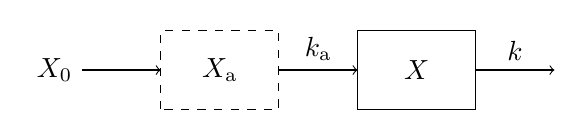
\begin{tikzpicture}
            \draw[->] (0,0) node[left]{$X_0$} --  (1,0);
            \draw[dashed] (1,-0.5) rectangle (2.5,0.5) node[midway] {$X_\mathrm{a}$};
            \draw[->] (2.5,0) -- (3.5,0) node[above,midway]{$k_\mathrm{a}$};
            \draw (3.5,-0.5) rectangle (5,0.5) node[midway] {$X$};
            \draw[->] (5,0) -- (6,0) node[above,midway]{$k$};
        \end{tikzpicture}
    \end{center}
    $X_0$为给药剂量；

    $X_\mathrm{a}$为吸收部位可被吸收进入血的药量；

    $k_\mathrm{a}$为一级吸收速率常数；
    
    $X$为体内药量；
    
    $k$为一级消除速率常数。
\end{frame}


\begin{frame}
    \frametitle{血药浓度与时间的关系}
    \begin{center}
        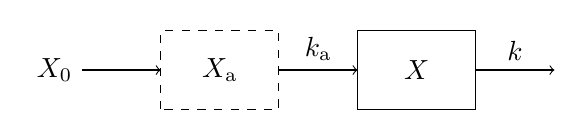
\begin{tikzpicture}
            \draw[->] (0,0) node[left]{$X_0$} --  (1,0);
            \draw[dashed] (1,-0.5) rectangle (2.5,0.5) node[midway] {$X_\mathrm{a}$};
            \draw[->] (2.5,0) -- (3.5,0) node[above,midway]{$k_\mathrm{a}$};
            \draw (3.5,-0.5) rectangle (5,0.5) node[midway] {$X$};
            \draw[->] (5,0) -- (6,0) node[above,midway]{$k$};
        \end{tikzpicture}
    \end{center}
    在血管外给药的一级吸收模型中 ， 吸收部位药量的变化速率与吸收部位的药量成正比：
    \[
        \frac{\mathrm{d}X_{\mathrm{a}}}{\mathrm{d}t}=-k_{\mathrm{a}}X_{\mathrm{a}}
    \]
    经拉氏变换得
    \[
        S\overline{X}_{\mathrm{a}}-FX_{0}=-k_{a}\overline{X}_{a}
    \]
    由于血管外给药吸收不一定充分 ， 因此 ， 给药部位可被吸收进入体内的药量应为给药剂量乘以吸收率$F$ 。
    \[
        \overline{X}_{a}=\frac{FX_0}{s+k_{\mathrm{a}}}
    \]
\end{frame}


\begin{frame}
    \frametitle{血药浓度与时间的关系}
    \begin{center}
        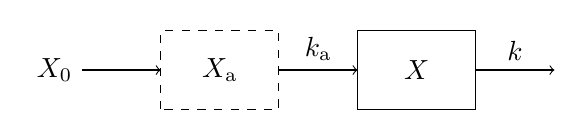
\begin{tikzpicture}
            \draw[->] (0,0) node[left]{$X_0$} --  (1,0);
            \draw[dashed] (1,-0.5) rectangle (2.5,0.5) node[midway] {$X_\mathrm{a}$};
            \draw[->] (2.5,0) -- (3.5,0) node[above,midway]{$k_\mathrm{a}$};
            \draw (3.5,-0.5) rectangle (5,0.5) node[midway] {$X$};
            \draw[->] (5,0) -- (6,0) node[above,midway]{$k$};
        \end{tikzpicture}
    \end{center}
    体内药量的变化速率则等于吸收速率与消除速率的代数和 ， 即 ：
    \[
        \frac{\mathrm{d}X}{\mathrm{d}t}=k_{\mathrm{a}}X_{\mathrm{a}}-kX
    \]
    经拉氏变换得
    \[
        s\overline{X}=k_{\mathrm{a}}\overline{X}_{\mathrm{a}}-k\overline{X}
    \]
    将$\overline{X}_{a}=\frac{FX_0}{s+k_{\mathrm{a}}}$代入，解得$\overline{X}$
    \[
        \overline{X}=\frac{k_{\mathrm{a}}FX_{0}}{(s+k)(s+k_{\mathrm{a}})}
    \]
    
\end{frame}


\begin{frame}
    \frametitle{血药浓度与时间的关系}
    经拉氏逆变换， 得到体内药量与时间的关系式 ：
    \[
        X=\frac{k_{a}FX_0}{k_{a}-k}(\mathrm{e}^{-kt}-\mathrm{e}^{-k_{a}t})
    \]
    将$X=CV$代入上式得单室模型药物血管外给药后，体内药物浓度$C$与时间$t$的关系式 ：
    \[
        C=\frac{k_{a}FX_0}{V(k_{a}-k)}(\mathrm{e}^{-kt}-\mathrm{e}^{-k_\mathrm{a}t})
    \]
    令$A=\frac{k_{a}FX_0}{V(k_{a}-k)}$，上式可简写为
    \[
        C=A(\mathrm{e}^{-kt}-\mathrm{e}^{-k_{a}t})
    \]
\end{frame}


\begin{frame}[t]
    \frametitle{}
    \begin{example}
        已知某单室模型药物口服的生物利用度为 70\%， 吸收速率常数$k_\mathrm{a}=0.8$ h$^{-1}$，消除速率常数$k$为 0.07h$^{-1}$， 表观分布容积$V$为10 L 。 若口服剂量为 200 mg ， 试求服药后3 h的血药浓度。若已知该药物在体内的最低有效血药浓度为8 $\mu$g/mL， 则什么时候第二次服药比较合适 ？
    \end{example}
\end{frame}


\begin{frame}
    \frametitle{药物动力学参数的计算}
    \begin{figure}[htpb]
        \centering
        
\includegraphics[width=.45\linewidth]{单室模型}
    \end{figure}
    \vspace{-1.5em}
    \begin{itemize}
      \item 峰左侧曲线称为吸收相 ， 此过程药物吸收速率大于消除速率 ， 反映了药物的吸收情况 ； 
      \item 峰的右侧称为消除相 ， 此过程药物吸收速率小于消除速率，反映了药物的消除情况 ；  
      \item 在到达峰顶的一瞬间 ， 吸收速率等于消除速率， 其峰值血药浓度就是峰浓度$C_\mathrm{max}$
      \item 达到峰浓度的时间称为达峰时间$t_\mathrm{max}$
    \end{itemize}
\end{frame}


\begin{frame}
    \frametitle{达峰时间}
    $C=\frac{k_{a}FX_0}{V(k_{a}-k)}(\mathrm{e}^{-kt}-\mathrm{e}^{-k_\mathrm{a}t})$对时间微分，得
    \[
        \frac{\mathrm{d}C}{\mathrm{d}t}=\frac{k_{\mathrm{a}}^{2}FX_{0}}{V(k_{a}-k)}\mathrm{e}^{-k_{a}t}-\frac{k_{\mathrm{a}}kFX_{0}}{V(k_{a}-k)}\mathrm{e}^{-kt}
    \]
    在$t_\mathrm{max}$时，$\frac{\mathrm{d}C}{\mathrm{d}t}=0$，
    \[
        \frac{k_\mathrm{a}^2FX_0}{V(k_\mathrm{a}-k)}\mathrm{e}^{-k_\mathrm{a}t_\mathrm{max}}=\frac{k_\mathrm{a}kFX_0}{V(k_\mathrm{a}-k)}\mathrm{e}^{-kt_\mathrm{max}}  \quad \text{化简得} \quad \frac{k_\mathrm{a}}k=\frac{\mathrm{e}^{-kt_\mathrm{max}}}{\mathrm{e}^{-k_\mathrm{a}t_\mathrm{max}}}
    \]
    解得
    \[
        t_{\mathrm{max}}=\frac{\ln k_{\mathrm{a}}-\mathrm{ln}k}{k_{\mathrm{a}}-k} \quad \text{或} \quad t_{\mathrm{max}}=\frac{2.303}{k_{\mathrm{a}}-k}\mathrm{lg}\frac{k_{\mathrm{a}}}{k}
    \]
    药物的$t_\mathrm{max}$由吸收速率常数$k_{\mathrm{a}}$和消除速率常数$k$决定 ， 与剂量大小无关 。 若消除速率常数$k$不变 ， 吸收速率常数$k_{\mathrm{a}}$增大 ， 达峰时间缩短 。
\end{frame}


\begin{frame}
    \frametitle{峰浓度}
    将$t_\mathrm{max}$代回式中， 可求得最大血药浓度 ：
    \[
        C_{\mathrm{max}}=\frac{k_{\mathrm{a}}FX_{0}}{V(k_{{a}}-k)}(\mathrm{e}^{-kt_{{max}}}-\mathrm{e}^{-k_{{a}}t_{{\mathrm{max}}}})
    \]
    将$\frac{k_\mathrm{a}}k=\frac{\mathrm{e}^{-kt_\mathrm{max}}}{\mathrm{e}^{-k_\mathrm{a}t_\mathrm{max}}}$代入，得
    \[
        C_{\mathrm{max}}=\frac{FX_{0}}{V}\mathrm{e}^{-kt_{\mathrm{max}}}
    \]
    可见 ，$C_\mathrm{max}$与$X_{0}$成正比 。 
    \begin{blankblock}{}
        药物制剂的达峰时间$t_\mathrm{max}$和峰浓度$C_\mathrm{max}$分别反映制剂中药物吸收的速度和程度 。 如果口服固体制剂在胃肠道中能很快崩解和较快地被吸收 ， 一般情况下达峰时间短 、 峰值血药浓度高 。
    \end{blankblock}
    
\end{frame}


\begin{frame}
    \frametitle{血药浓度-时间曲线下面积}
    血药浓度-时间曲线下面积$AUC$的大小反映药物吸收入血的相对量 ， 它可由血药浓度的时间函数式从时间$0\to \infty$内定积分求得 ， 即 ：
    \[
        AUC_{0\to\infty}=\int_0^\infty C\mathrm{d}t=\int_0^\infty\frac{k_aFX_0}{V(k_a-k)}(\mathrm{e}^{-kt}-\mathrm{e}^{-k_\mathrm{a}t})\mathrm{d}t
    \]
    运算后，得
    \[
        AUC_{0\to\infty}=\frac{FX_{0}}{kV}
    \]
\end{frame}


\begin{frame}
    \frametitle{梯形法求$AUC_{0\to\infty}$}
\end{frame}


\begin{frame}[t]
    \frametitle{}
    \begin{example}
        已知大鼠口服单室模型药物蒿苯酯的$k_\mathrm{a}=1.905$ \si{h^{-1}}，$k=0.182$ \si{h^{-1}}，$V=4.25$ \si{L}，$F=0.80$，如口服剂量为150 mg ， 试计算$t_\mathrm{max}$、$C_\mathrm{max}$及$AUC_{0\to\infty}$。
    \end{example}
\end{frame}


\begin{frame}
    \frametitle{残数法求消除速率常数$k$和吸收速率常数$k_\mathrm{a}$}
    若$k_\mathrm{a}\gg k$，当$t$充分大时 ，$\mathrm{e}^{-k_\mathrm{a}t}$首先趋于零 ， 则式$C=\frac{k_{a}FX_0}{V(k_{a}-k)}(\mathrm{e}^{-kt}-\mathrm{e}^{-k_\mathrm{a}t})$简化为 ：
    \[
        C=\frac{k_{a}FX_0}{V(k_{a}-k)}\mathrm{e}^{-kt}
    \]
    两边取常用对数，
    \[
        \lg C=-\frac{k}{2.303}t+\lg\frac{k_{\mathrm{a}}FX_{0}}{V(k_{\mathrm{a}}-k)}
    \]
    两边取自然对数，
    \[
        \ln C=-kt+\ln\frac{k_{\mathrm{a}}FX_{0}}{V(k_{\mathrm{a}}-k)}
    \]
    以血药浓度的对数对时间作图得一条二项指数曲线 ，其尾段为一条直线 ，从直线的斜率可求出总消除速率常数值 ；若$F$、$V$已知 ， 从该直线外推至零时间的截距可求出$k_{\mathrm{a}}$。
\end{frame}


\begin{frame}
    \frametitle{}
    \begin{figure}[htpb]
        \centering
        
\includegraphics[width=.85\linewidth]{残数法}
        \caption{单室模型药物血管外给药后的血药浓度、残数浓度-时间半对数图}
    \end{figure}
\end{frame}


\begin{frame}
    \frametitle{残数法求消除速率常数$k$和吸收速率常数$k_\mathrm{a}$}
    如果$F$、$V$是未知的 ， 此时可应用残数法求出吸收速率常数$k_{\mathrm{a}}$。 方法如下 ：
    
    $C=\frac{k_{a}FX_0}{V(k_{a}-k)}(\mathrm{e}^{-kt}-\mathrm{e}^{-k_\mathrm{a}t})$移项，得
    \[
        \frac{k_{a}FX_0}{V(k_{a}-k)}\mathrm{e}^{-kt} - C = \frac{k_{a}FX_0}{V(k_{a}-k)}\mathrm{e}^{-k_\mathrm{a}t}
    \]
    等式左端为$t$时刻消除相尾段直线的外推值减$t$时刻血药浓度的实测值，记作\highlight{残差浓度$C_{\mathrm{r}}$}
    
    两边取对数，得：
    \[
        \lg C_{r}=-\frac{k_{\mathrm{a}}}{2.303}t+\lg\frac{k_\mathrm{a}FX_{0}}{V(k_\mathrm{a}-k)} \quad \text{或} \quad \ln C_{r}=-k_{\mathrm{a}}t+\ln\frac{k_\mathrm{a}FX_{0}}{V(k_\mathrm{a}-k)}
    \]
    以血药浓度的对数对时间作图得一条直线 ，从直线的斜率可求出吸收速率常数$k_{\mathrm{a}}$；若$F$、$X_0$已知 ， 从截距可求出$V$。
\end{frame}


\begin{frame}
    \frametitle{残差法步骤}
    \begin{enumerate}
      \item 根据$\ln C-t$数据 ， 采用线性回归求得消除相尾段直线回归方程，根据斜率求得消除速率常数$k$，消除半衰期$t_{1/2}$
      \item 将吸收相中的时间点代入消除相尾段直线回归方程 ， 求得该时间点在尾端直线外推线上的血药浓度值
      \item 用外推血药浓度值减去吸收相中同一时间点的实测血药浓度值，即得一系列残数浓度值$C_{\mathrm{r}}$
      \item 根据$\ln C_{\mathrm{r}}-t$数据 ， 采用线性回归求得残数线回归方程，根据斜率求得吸收速率常数$k_{\mathrm{a}}$，吸收半衰期$t_{{1/2\alpha}}$
      \item 若已知$F$、$X_0$，根据残数线截距可求出$V$值
    \end{enumerate}
\end{frame}


\begin{frame}
    \frametitle{残差法要求}
    \begin{enumerate}
      \item 药物的吸收必须符合一级速率过程
      \item $k_\mathrm{a}\gg k$
      \item 取样时间$t$应充分长， 这样才能使$\mathrm{e}^{-k_\mathrm{a}t}\to 0$
      \item 用残数法求$k_{\mathrm{a}}$，必须在吸收相内测定足够的数据 ， 一般不少于 3 个时间点。
    \end{enumerate}
    \begin{blankblock}{}
        大多数药物满足此条件 。 因为一般药物制剂的吸收半衰期总是短于消除半衰期，但缓释剂型和一些难吸收的药物除外。
    \end{blankblock}
\end{frame}


\begin{frame}[t]
    \frametitle{}
    \begin{example}
        口服单室模型药物100 mg的溶液剂后 ， 测得各时间的血药浓度如下 ， 试求该药物的$k$、 $t_{1/2}$及$k_\mathrm{a}$、 $t_{1/2\alpha}$值 。
        \begin{table}
            \centering
            \small
            \begin{tabular}{cccccccccccc}
                \bottomrule
                $t$(h) & 0.5 & 1.0 & 2.0 & 4.0 & 8.0 & 12.0 & 18.0 & 24.0 & 36.0 & 48.0 & 72.0 \hspace{-9pt} \\ \hline
                $C$($\mu$g/mL) & 5.36 & 9.95 & 17.18 & 25.78 & 29.78 & 26.63 & 19.40 & 13.26 & 5.88 & 2.56 & 0.49 \hspace{-9pt} \\ \toprule 
            \end{tabular}
        \end{table}
    \end{example}
\end{frame}


\begin{frame}
    \frametitle{Wagner-Nelson 法求$k_\mathrm{a}$}
    Wagner-Nelson法，简称W-N法 ， 也称为待吸收分数法 ， 是求算吸收速率常数的经典方法 。 Wagner-Nelson 法求算吸收速率常数对吸收模型无要求 ，但对药动学模型有要求 ， 主要适用于单室模型药物 。 

    在口服给药后的任一时刻 ， 机体已吸收的药量$X_\mathrm{A}$， 等于该时刻的体内药量$X$与该时刻的累积消除药量$X_\mathrm{E}$之和 ：
    \[
        X_\mathrm{A} = X + X_\mathrm{E}
    \]
    对时间$t$微分，得
    \[
        \frac{\mathrm{d}X_{\mathrm{A}}}{\mathrm{d}t}=\frac{\mathrm{d}X}{\mathrm{d}t}+\frac{\mathrm{d}X_{\mathrm{E}}}{\mathrm{d}t}
    \]
    药物在体内的消除符合一级速率过程 ， 故上式中$\frac{\mathrm{d}X_{\mathrm{E}}}{\mathrm{d}t}=kX$：
    \[
        \frac{\mathrm{d}X_{\mathrm{A}}}{\mathrm{d}t}=\frac{\mathrm{d}X}{\mathrm{d}t}+kX
    \]
\end{frame}


\begin{frame}
    \frametitle{Wagner-Nelson 法求$k_\mathrm{a}$}
    \begin{minipage}{0.48\linewidth}
        因$X=VC$：
    \[
        \frac{\mathrm{d}X_{\mathrm{A}}}{\mathrm{d}t}=\frac{\mathrm{d}X}{\mathrm{d}t}+kVC
    \]
    在时间$0-t$内积分：
    \[
        (X_{\mathrm{A}})_{t}=VC_{t}+kV\int_{0}^{t}C\mathrm{d}t
    \]
    在时间$0-\infty$内积分：
    \[
        (X_{\mathrm{A}})_{\infty}=kV\int_{0}^{\infty}C\mathrm{d}t
    \]
    两式相除，得：
    \[
        \frac{(X_{\mathrm{A}})_{t}}{(X_{\mathrm{A}})_{\infty}}=\frac{C_{t}+k\int_{0}^{t}C\mathrm{d}t}{k\int_{0}^{\infty}C\mathrm{d}t}
    \]
    \end{minipage}\hfill
    \begin{minipage}{0.48\linewidth}
        \begin{itemize}
          \item[$(X_{\mathrm{A}})_{t}$] \ 给药后$t$时刻吸收的药物量
          \item[$C_{t}$：] \ $t$时刻的血药浓度
          \item[$\int_{0}^{t}C\mathrm{d}t$：] \ $0-t$血药浓度-时间曲线下面积
          \item[$(X_{\mathrm{A}})_{\infty}$：] \ 吸收的总药量
          \item[$\int_{0}^{\infty}C\mathrm{d}t$：] \ 血药浓度-时间曲线下总面积
          \item[$\frac{(X_{\mathrm{A}})_{t}}{(X_{\mathrm{A}})_{\infty}}$：] \ 药物吸收分数，给药后$t$时间内已吸收的药物量占全部吸收药物量的比
        \end{itemize}
    \end{minipage}
    
\end{frame}


\begin{frame}
    \frametitle{Wagner-Nelson 法求$k_\mathrm{a}$}
    \[
        \begin{aligned}
            C_{t}+k\int_{0}^{t}C\mathrm{d}t& =\frac{k_{a}FX_{0}}{V(k_{a}-k)}(\mathrm{e}^{-kt}-\mathrm{e}^{-k_{a}t})+k\int_{0}^{t}\frac{k_{a}FX_{0}}{V(k_{a}-k)}(\mathrm{e}^{-kt}-\mathrm{e}^{-k_{a}t})\mathrm{d}t  \\
            &=\frac{k_{a}FX_{0}}{V(k_{a}-k)}[(\mathrm{e}^{-kt}-\mathrm{e}^{-k_{a}t})+k\int_{0}^{t}(\mathrm{e}^{-kt}-\mathrm{e}^{-k_{a}t})\mathrm{d}t] \\
            &=\frac{k_{a}FX_{0}}{V(k_{\mathrm{a}}-k)}\left[(\mathrm{e}^{-kt}-\mathrm{e}^{-k_{a}t})+k\left(\left.\frac{\mathrm{e}^{-kt}}{-k}\right|_{0}^{t}-\left.\frac{\mathrm{e}^{-k_{a}t}}{-k_{a}}\right|_{0}^{t}\right)\right] \\            
            &=\frac{k_{a}FX_{0}}{V(k_{a}-k)}\left\{\left(\mathrm{e}^{-kt}-\mathrm{e}^{-k_{a}t}\right)+k\left[(\frac{\mathrm{e}^{-kt}}{-k}-\frac{1}{-k})-(\frac{\mathrm{e}^{-k_{a}t}}{-k_{a}}-\frac{1}{-k_{a}})\right]\right\} \\
            &=\frac{k_{\mathrm{a}}FX_{0}}{V(k_{\mathrm{a}}-k)}\left[\frac{k_{\mathrm{a}}-k}{k_{\mathrm{a}}}(1-\mathrm{e}^{-k_{a}t})\right] \\
            &=\frac{FX_0}V(1-\mathrm{e}^{-k_at})
            \end{aligned}
    \]
\end{frame}


\begin{frame}
    \frametitle{Wagner-Nelson 法求$k_\mathrm{a}$}
    将$C_{t}+k\int_{0}^{t}C\mathrm{d}t=\frac{FX_0}V(1-\mathrm{e}^{-k_\mathrm{a}t})$，$\int_{0}^{\infty}C\mathrm{d}t=\frac{FX_{0}}{kV}$代入$\frac{(X_{\mathrm{A}})_{t}}{(X_{\mathrm{A}})_{\infty}}=\frac{C_{t}+k\int_{0}^{t}C\mathrm{d}t}{k\int_{0}^{\infty}C\mathrm{d}t}$，得
    \[
        \frac{(X_{\mathrm{A}})_{t}}{(X_{\mathrm{A}})_{\infty}}=1-\mathrm{e}^{-k_\mathrm{a}t}
    \]
    即
    \[
        1-\frac{(X_{\mathrm{A}})_{t}}{(X_{\mathrm{A}})_{\infty}}=\mathrm{e}^{-k_\mathrm{a}t}
    \]
    两边取对数，得
    \[
        \lg\left[1-\frac{\left(X_{\mathrm{A}}\right)_t}{\left(X_{\mathrm{A}}\right)_{\mathrm{\infty}}}\right]=-\frac{k_{\mathrm{a}}}{2.303}t \quad \text{或} \quad \ln\left[1-\frac{\left(X_{\mathrm{A}}\right)_t}{\left(X_{\mathrm{A}}\right)_{\mathrm{\infty}}}\right]=-kt
    \]
    $\left[1-\frac{\left(X_{\mathrm{A}}\right)_t}{\left(X_{\mathrm{A}}\right)_{\mathrm{\infty}}}\right]$为待吸收分数，以其对数对$t$作图得一直线，由直线的斜率求得$k_\mathrm{a}$。
\end{frame}


\begin{frame}
    \frametitle{Wagner-Nelson 法求$k_\mathrm{a}$的步骤}
    \begin{enumerate}
      \item 选用尾段消除相的实测浓度-时间数据，以浓度对数对$t$作图，采用线性回归法求得尾段直线回归方程 ， 根据直线斜率求得消除速率常数$k$。
      \item 根据实测浓度-时间数据，用梯形法分别求得从0到$t$时间点的$AUC_{0\to t_i}$以及$C{_t{_i}}+k\int_{0}^{t_i}C\mathrm{d}t=C_t{_i}+kAUC_{0\to t_i}$
      \item 根据最后一点实测血药浓度$C_\mathrm{n}$与$k$值，求得$k\int_{0}^{\infty}C\mathrm{d}t=k(AUC_{0\to t_n}+AUC_{t_n\to\infty})=k\cdot AUC_{0\to t_n}+C_n$
      \item 计算$t{_i}$时间点的药物吸收分数
      \item 计算$t{_i}$时间点的待吸收分数，以其对数对$t$作图，求得直线回归方程，根据直线的斜率求得吸收速率常数$k_\mathrm{a}$
    \end{enumerate}
\end{frame}


\begin{frame}[t]
    \frametitle{}
    \begin{example}
        口服单室模型药物100 mg的溶液剂后 ， 测得各时间的血药浓度如下 ， 用Wagner-Nelson 法求$k_\mathrm{a}$。
        \begin{table}
            \centering
            \small
            \begin{tabular}{cccccccccccc}
                \bottomrule
                $t$(h) & 0.5 & 1.0 & 2.0 & 4.0 & 8.0 & 12.0 & 18.0 & 24.0 & 36.0 & 48.0 & 72.0 \hspace{-9pt} \\ \hline
                $C$($\mu$g/mL) & 5.36 & 9.95 & 17.18 & 25.78 & 29.78 & 26.63 & 19.40 & 13.26 & 5.88 & 2.56 & 0.49 \hspace{-9pt} \\ \toprule 
            \end{tabular}
        \end{table}
    \end{example}
\end{frame}


\begin{frame}[t]
    \frametitle{}
    \begin{question}
        口服某单室模型药物50 mg的混悬剂后 ， 测得各时间的血药浓度如下 ， 用Wagner-Nelson 法求$k_\mathrm{a}$。
        \begin{table}
            \centering
            \small
            \begin{tabular}{cccccccccccc}
                \bottomrule
                $t$(h) & 0.5 & 1.0 & 2.0 & 4.0 & 8.0 & 12.0 & 18.0 & 24.0 & 36.0 & 48.0 & 72.0 \hspace{-9pt} \\ \hline
                $C$($\mu$g/mL) & 2.68 & 4.98 & 8.59 & 12.89 & 14.89 & 13.32 & 9.70 & 6.63 & 2.94 & 1.28 & 0.24 \hspace{-9pt} \\ \toprule 
            \end{tabular}
        \end{table}
    \end{question}
\end{frame}



\begin{frame}
    \frametitle{滞后时间}
    血管外给药后，药物往往要经过一段时间才能吸收进入血液循环。从给药开始到血液中出现药物所需要的时间，称为滞后时间，常用$t_\mathrm{lag}$或$t_0$表示。

    若$t_\mathrm{lag}$超过一定数值，则在药物动力学参数计算时应对时间数据进行校正。

    对于单室模型血管外给药，考虑滞后时间后，体内药物浓度$C$与时
    间$t$的关系式可改写为：
    \[
        C=\frac{k_\mathrm{a}FX_0}{V(k_\mathrm{a}-k)}\Big[\mathrm{e}^{-k(t-t_{\mathrm{lag}})}-\mathrm{e}^{-k_\mathrm{a}(t-t_\mathrm{lag})}\Big]
    \]
    滞后时间的求法：
    \begin{enumerate}
      \item 图解法
      \item 参数计算法
      \item 抛物线法
    \end{enumerate}
\end{frame}


\begin{frame}
    \frametitle{图解法}
    过血药浓度对数--时间（$\lg C-t$）曲线的尾段直线的外推线与残数线的交点，作横轴（时间轴）的垂线，垂足所对应的时间便为$t_\mathrm{lag}$。
    \begin{figure}[htpb]
        \centering
        
\includegraphics[width=.6\linewidth]{tlag}
    \end{figure}
\end{frame}


\begin{frame}
    \frametitle{参数计算法}
    此法原理与图解法相同。

    外推线与残数线的方程分别为
    \[
        \ln C=-kt+\ln A_1
    \]
    \[
        \ln C_{r}=-k_\mathrm{a}t+\ln A_2
    \]
    当$\ln C = \ln C_{r}$时，此时的时间即为$t_\mathrm{lag}$，故有：
    \[
        -kt_{\mathrm{lag}}+\ln A_{1}=-k_\mathrm{a}t_{\mathrm{lag}}+\ln A_{2}
    \]
    整理，得
    \[
        t_{\mathrm{lag}}=\frac{\ln A_{2} - \ln A_{1}}{k_{\mathrm{a}}-k}
    \]
\end{frame}


\begin{frame}[t]
    \frametitle{}
    \begin{example}
        口服单室模型药物100 mg的溶液剂后 ， 测得各时间的血药浓度如下 ， 计算滞后时间。
        \begin{table}
            \centering
            \small
            \begin{tabular}{cccccccccccc}
                \bottomrule
                $t$(h) & 0.5 & 1.0 & 2.0 & 4.0 & 8.0 & 12.0 & 18.0 & 24.0 & 36.0 & 48.0 & 72.0 \hspace{-9pt} \\ \hline
                $C$($\mu$g/mL) & 5.36 & 9.95 & 17.18 & 25.78 & 29.78 & 26.63 & 19.40 & 13.26 & 5.88 & 2.56 & 0.49 \hspace{-9pt} \\ \toprule 
            \end{tabular}
        \end{table}
    \end{example}
\end{frame}


\subsection{尿药排泄的经时变化}


\begin{frame}
    \frametitle{尿药排泄速率与时间的关系（速度法）}
    血管外给药后若大部分药物以原形从尿中排出，且药物经肾排泄符合一级速率过程，则尿药排泄速率与当时体内的药量成正比：
    \[
        \frac{\mathrm{d}X_\mathrm{u}}{\mathrm{d}t}=k_\mathrm{e}X
    \]
    将$X=\frac{k_\mathrm{a}FX_0}{k_\mathrm{a}-k}(\mathrm{e}^{-kt}-\mathrm{e}^{-k_\mathrm{a}t})$代入，得
    \[
        \frac{\mathrm{d}X_\mathrm{u}}{\mathrm{d}t}=k_\mathrm{e}X=\frac{k_\mathrm{e}k_\mathrm{a}FX_0}{k_\mathrm{a}-k}(\mathrm{e}^{-kt}-\mathrm{e}^{-k_\mathrm{a}t})
    \]
    若$k_\mathrm{a}\gg k$，当$t \to \infty$，$\mathrm{e}^{-k_\mathrm{a}t} \to 0$， 上式简化为
    \[
        \frac{\mathrm{d}X_\mathrm{u}}{\mathrm{d}t}=\frac{k_\mathrm{e}k_\mathrm{a}FX_0}{k_\mathrm{a}-k}\mathrm{e}^{-kt}
    \]
\end{frame}


\begin{frame}
    \frametitle{尿药排泄速率与时间的关系（速度法）}
    上式两边取对数，得
    \[
        \ln \frac{\mathrm{d}X_\mathrm{u}}{\mathrm{d}t}=-kt + \ln \frac{k_\mathrm{e}k_\mathrm{a}FX_0}{k_\mathrm{a}-k}
    \]
    与静脉注射给药的尿药排泄数据处理方法一样，以$\frac{\Delta X_{\mathrm{u}}}{\Delta t}$代替$\frac{\mathrm{d}X_\mathrm{u}}{\mathrm{d}t}$，以$t_\mathrm{c}$代替$t$，以$\frac{\Delta X_{\mathrm{u}}}{\Delta t}$的对数对$t_\mathrm{c}$作图，从直线的斜率可求出消除速率常数$k$值。
\end{frame}


\begin{frame}
    \frametitle{尿药排泄总量}
    \[
        \frac{\mathrm{d}X_\mathrm{u}}{\mathrm{d}t}=\frac{k_\mathrm{e}k_\mathrm{a}FX_0}{k_\mathrm{a}-k}(\mathrm{e}^{-kt}-\mathrm{e}^{-k_\mathrm{a}t})
    \]
    对上式从$0 \to \infty$积分，得到尿药排泄总量：
    \[
        X_\mathrm{u}^\infty = \int_0^\infty \frac{k_\mathrm{e}k_\mathrm{a}FX_0}{k_\mathrm{a}-k}(\mathrm{e}^{-kt}-\mathrm{e}^{-k_\mathrm{a}t}) \dif t = \frac{k_\mathrm{e}FX_0}{k}
    \]
\end{frame}


\begin{frame}
    \frametitle{集尿结束后的剩余尿药排泄量}
    \[
        \frac{\mathrm{d}X_\mathrm{u}}{\mathrm{d}t}=\frac{k_\mathrm{e}k_\mathrm{a}FX_0}{k_\mathrm{a}-k}(\mathrm{e}^{-kt}-\mathrm{e}^{-k_\mathrm{a}t})
    \]
    对上式从$t \to \infty$积分，得：
    \[
        (X_\mathrm{u})_{t \to \infty} = \int_t^\infty \frac{k_\mathrm{e}k_\mathrm{a}FX_0}{k_\mathrm{a}-k}(\mathrm{e}^{-kt}-\mathrm{e}^{-k_\mathrm{a}t}) \dif t
    \]
    若$k_\mathrm{a}\gg k$，当$t$足够大时，$\mathrm{e}^{-k_\mathrm{a}t} \to 0$，上式可简化为
    \[
        (X_\mathrm{u})_{t \to \infty} = \frac{k_\mathrm{e}k_\mathrm{a}FX_0}{k_\mathrm{a}-k}\int_t^\infty \mathrm{e}^{-kt} \dif t = \frac{k_\mathrm{e}k_\mathrm{a}FX_0}{k_\mathrm{a}-k}\cdot \frac{\mathrm{e}^{-kt}}{k}
    \]
    将最后一点$t$的尿药排泄速率$(\frac{\mathrm{d}X_\mathrm{u}}{\mathrm{d}t})_t=\frac{k_\mathrm{e}k_\mathrm{a}FX_0}{k_\mathrm{a}-k}\mathrm{e}^{-kt}$代入上式，得剩余尿药排泄量：
    \[
        (X_\mathrm{u})_{t \to \infty} = \frac{(\mathrm{d}X_\mathrm{u}/\mathrm{d}t)_t}{k}
    \]
\end{frame}


\begin{frame}[t]
    \frametitle{}
    \begin{example}
        某抗生素为单室模型药物 ， 单次口服 250 mg 后 ， 于各时间段收集尿样 ， 测定各时间段的尿药量 ， 实验数据如下表所示。 求消除速率常数$k$，消除半衰期$t_{1/2}$以及尿药排泄百分数。
        \begin{table}
            \centering
            \small
            \begin{tabular}{cccccccccccc}
                \bottomrule
                $t$(h) & 1.0 & 2.0 & 3.0 & 6.0 & 10.0 & 15.0 & 24.0  \\ \hline
                $\Delta X_\mathrm{u}$(mg) & 4.12 & 5.26 & 5.98 & 17.86 & 14.30 & 8.32 & 4.88 \hspace{-9pt} \\ \toprule 
            \end{tabular}
        \end{table}
    \end{example}
\end{frame}


\begin{frame}
    \frametitle{尿药排泄量与时间的关系}
    \[
        \frac{\mathrm{d}X_\mathrm{u}}{\mathrm{d}t}=\frac{k_\mathrm{e}k_\mathrm{a}FX_0}{k_\mathrm{a}-k}(\mathrm{e}^{-kt}-\mathrm{e}^{-k_\mathrm{a}t})
    \]
    积分，得
    \[
        X_\mathrm{u}=\frac{k_\mathrm{e}k_\mathrm{a}FX_0}{k}\Big[\frac{1}{k_\mathrm{a}}+\frac{\mathrm{e}^{-kt}}{k-k_\mathrm{a}}-\frac{k\mathrm{e}^{-k_\mathrm{a}t}}{k_\mathrm{a}(k-k_\mathrm{a})}\Big]
    \]
    将$X_\mathrm{u}^\infty = \frac{k_\mathrm{e}FX_0}{k}$代入，得
    \[
        X_\mathrm{u}=X_\mathrm{u}^\infty k_\mathrm{a}\Big[\frac{1}{k_\mathrm{a}}+\frac{\mathrm{e}^{-kt}}{k-k_\mathrm{a}}-\frac{k\mathrm{e}^{-k_\mathrm{a}t}}{k_\mathrm{a}(k-k_\mathrm{a})}\Big]
    \]
\end{frame}


\begin{frame}
    \frametitle{残数法求消除速率常数$k$}
    \[
        X_\mathrm{u}^\infty - X_\mathrm{u} = \frac{X_\mathrm{u}^\infty}{k_\mathrm{a} - k}(k_\mathrm{a}\mathrm{e}^{-kt} - k\mathrm{e}^{-k_\mathrm{a}t})
    \]
    一般情况下，$k_\mathrm{a}\gg k$，当$t$足够大时，$\mathrm{e}^{-k_\mathrm{a}t}$首先趋于0：
    \[
        X_\mathrm{u}^\infty - X_\mathrm{u} = \frac{X_\mathrm{u}^\infty k_\mathrm{a}}{k_\mathrm{a} - k}\mathrm{e}^{-kt}
    \]
    两边取对数
    \[
        \ln{(X_\mathrm{u}^\infty - X_\mathrm{u})} = -kt + \ln {\frac{X_\mathrm{u}^\infty k_\mathrm{a}}{k_\mathrm{a} - k}}
    \]
    以$\ln{(X_\mathrm{u}^\infty - X_\mathrm{u})}$对$t$作图，由尾段直线的斜率可求出消除速率常数$k$。
\end{frame}


\begin{frame}
    \frametitle{残数法求吸收速率常数$k_\mathrm{a}$}
    $k_\mathrm{a}\gg k$时，根据$X_\mathrm{u}^\infty - X_\mathrm{u} = \frac{X_\mathrm{u}^\infty}{k_\mathrm{a} - k}(k_\mathrm{a}\mathrm{e}^{-kt} - k\mathrm{e}^{-k_\mathrm{a}t})$求残数亏量值：
    \[
        \frac{X_\mathrm{u}^\infty}{k_\mathrm{a} - k} k_\mathrm{a}\mathrm{e}^{-kt} - (X_\mathrm{u}^\infty - X_\mathrm{u}) = \frac{X_\mathrm{u}^\infty}{k_\mathrm{a} - k} k\mathrm{e}^{-k_\mathrm{a}t}
    \]
    其中，$\frac{X_\mathrm{u}^\infty}{k_\mathrm{a} - k} k_\mathrm{a}\mathrm{e}^{-kt}$为根据回归方程求得的吸收相$X_\mathrm{u}^\infty - X_\mathrm{u}$的外推值。

    两边取对数，并绘制残数线，根据直线的斜率即可求得吸收速率常数$k_\mathrm{a}$。
    \begin{blankblock}{}
        需要注意 ， 利用血管外给药后的尿药数据 ， 以残数法求吸收速率常数时 ， 必须在吸收相内收集足够的尿样 ， 这只有在药物吸收较慢时才有可能 。 由于多数药物吸收较快 ，在吸收相内不易获得较多的尿药数据 ， 难以精确求出 ， 因此采用尿药残数法求有局限性。
    \end{blankblock}
\end{frame}


\begin{frame}
    \frametitle{Wagner-Nelson法计算药物动力学参数}
    由$\frac{\mathrm{d}X_\mathrm{u}}{\mathrm{d}t}=k_\mathrm{e}X$，得
    \[
        X = \frac{1}{k_\mathrm{e}} \cdot \frac{\mathrm{d}X_\mathrm{u}}{\mathrm{d}t}
    \]
    代入式$\frac{\mathrm{d}X_\mathrm{A}}{\mathrm{d}t} = \frac{\mathrm{d}X}{\mathrm{d}t} + kX$，得
    \[
        \frac{\mathrm{d}X_\mathrm{A}}{\mathrm{d}t} = \frac{1}{k_\mathrm{e}} \cdot \frac{\dif (\mathrm{d}X_\mathrm{u}/\mathrm{d}t)}{\mathrm{d}t} + \frac{k}{k_\mathrm{e}} \cdot \frac{\mathrm{d}X_\mathrm{u}}{\mathrm{d}t}
    \]
    上式从$0 \to t$积分，得
    \[
        (X_\mathrm{A})_t = \frac{1}{k_\mathrm{e}} \left(\frac{\mathrm{d}X_\mathrm{u}}{\mathrm{d}t}\right)_t + \frac{k}{k_\mathrm{e}}(X_\mathrm{u})_t
    \]
    当$t \to \infty$时，$(\mathrm{d}X_\mathrm{u}/\mathrm{d}t) \to 0$，上式可写成
    \[
        (X_\mathrm{A})_\infty = \frac{k}{k_\mathrm{e}}X_\mathrm{u}^\infty
    \]
\end{frame}


\begin{frame}
    \frametitle{Wagner-Nelson法计算药物动力学参数}
    \[
        \frac{(X_\mathrm{A})_t}{(X_\mathrm{A})_\infty} = \frac{(\mathrm{d}X_\mathrm{u}/\mathrm{d}t)_t + k(X_\mathrm{u})_t}{kX_\mathrm{u}^\infty}
    \]
    由上式可见 ， 根据尿药排泄数据也可求得待吸收分数$1-\frac{(X_\mathrm{A})_t}{(X_\mathrm{A})_\infty}$。
    
    对于单室模型药物血管外给药 ， 以$\ln \left[1-\frac{(X_\mathrm{A})_t}{(X_\mathrm{A})_\infty}\right]$对$t$作图为过原点的直线，斜率为$-k_\mathrm{a}$。

    实际应用时 ， 用$\frac{\Delta X_\mathrm{u}}{\Delta t}$代替$\frac{\dif X_\mathrm{u}}{\dif t}$，用两次集尿期的中点时间$t_\mathrm{c}$代替$t$， 得 ：
    \[
        \frac{(X_\mathrm{A})_t}{(X_\mathrm{A})_\infty} = \frac{\frac{1}{k}(\Delta X_\mathrm{u}/\Delta t)_t + (X_\mathrm{u})_t}{X_\mathrm{u}^\infty}
    \]
\end{frame}


\begin{frame}[t]
    \frametitle{}
    \begin{example}
        口服某单室模型药物后 ， 于不同时间收集尿液 ， 测得尿中累积药量$X_\mathrm{u}$如下 ， 求该药物的吸收速率常数$k_\mathrm{a}$。
        \begin{table}
            \centering
            \small
            \begin{tabular}{cccccccccccc}
                \bottomrule
                $t$(h) & 1 & 2 & 3 & 4 & 6 & 8 & 10 & 12  &  16 & 20  & 24 \\ \hline
                $X_\mathrm{u}$(mg) & 10 & 23 & 46 & 66 & 119 & 166 & 206 & 242 & 293 & 325 & 352  \\ \toprule 
            \end{tabular}
        \end{table}
    \end{example}
\end{frame}


\subsection{血药浓度与尿药浓度的关系}


\begin{frame}
    \frametitle{血药浓度与尿药浓度的关系}
    \begin{figure}[htpb]
        \centering
        
\includegraphics[width=.9\linewidth]{血药尿药关系}
    \end{figure}
\end{frame}



\end{document}